\documentclass[12pt, a4paper]{scrreprt}

\renewcommand*\familydefault{\sfdefault} 
%\usepackage[T1]{fontenc}

\usepackage[english]{babel}
%\usepackage{cite}
\usepackage[utf8]{inputenc}
%\usepackage[onehalfspacing]{setspace}
\usepackage{geometry, textcomp}
\newgeometry{right=2cm,left=4cm, top=2.5cm, bottom=2.3cm, footnotesep=0.5cm}
%\usepackage[acronym]{glossaries}

\usepackage[printonlyused]{acronym}  % Abkürzungsverzeichnis [nur verwendete Abkürzugen]

%\glsenablehyper

%\makeglossaries

\usepackage{savesym}
\usepackage{amsmath,amssymb,amstext}
\savesymbol{iint}
\usepackage{txfonts}

\restoresymbol{TXF}{iint}
\usepackage[automark,headsepline,ilines,komastyle]{scrpage2}
\usepackage{blindtext}
\usepackage[euler]{textgreek}
\setlength{\parindent}{0pt}
\setlength{\headheight}{1.5\baselineskip}
\renewcommand{\baselinestretch}{1.5}

\pagestyle{scrheadings}
\clearscrheadfoot
\ihead[]{}
\chead[]{}
\ohead[]{\headmark \hfill \thepage}
\ifoot[]{}
\cfoot[]{}
\ofoot[]{}

\setheadsepline[\textwidth]{1pt}
\usepackage{tabularx}
\usepackage{colortbl}
\usepackage{multirow}
\usepackage{hhline}
\usepackage{array}
\usepackage{tocloft}
\usepackage[hidelinks]{hyperref}
\tocloftpagestyle{scrheadings}
\renewcommand{\chapterpagestyle}{scrheadings}
\usepackage[font=footnotesize]{caption}

\usepackage{tikz}
\usepackage{rotating} 

\newenvironment{packed_item}
	{\begin{itemize}
			\setlength{\itemsep}{0pt}
			\setlength{\topsep}{0pt}
			\setlength{\parsep}{0pt}
			\setlength{\parskip}{0pt}}
		{\end{itemize}}
	
\usepackage[style=authoryear, natbib=true, backend=biber]{biblatex}

\renewcommand{\nameyeardelim}{ }
\usepackage[babel,german=guillemets]{csquotes}

\makeatletter

\newrobustcmd*{\parentexttrack}[1]{%
	\begingroup
	\blx@blxinit
	\blx@setsfcodes
	\blx@bibopenparen#1\blx@bibcloseparen
	\endgroup}

\AtEveryCite{%
	\let\parentext=\parentexttrack%
	\let\bibopenparen=\bibopenbracket%
	\let\bibcloseparen=\bibclosebracket}

\makeatother

\usepackage{pstricks}
\usepackage{pstricks-add}

\bibliography{Lit.bib}

\usepackage[final]{pdfpages}

\begin{document}
		\begin{titlepage}
			\begin{center}
			\setlength{\headheight}{1.5\baselineskip}
			\renewcommand{\baselinestretch}{1.5}
					\textbf{\large FOM - Hochschule für Oekonomie \& Management \\
						Hamburg \\
						\ \\
						Master-Studiengang Big Data \& Business Analytics \\
						3. Semester \\
						\ \\
						Development of a chatbot to improve process of patient management and  \ \\		 documentation of diseases and their symptoms \ \\
						\ \\
						}
						
					\textrm{
						\ \\
						Betreuer: Prof. Dr. Kai Brüssau \\
						\ \\
						Autor: Jacqueline Franßen \\
						\ \\
						Matrikel-Nr: 496804 \\
						\ \\
						3. Fachsemester \\
						\ \\
						Hamburg, den 28.02.2020 \\
						}
			\end{center}
		\end{titlepage}

%\includepdf{Image/Deckblatt.pdf}

			\setcounter{tocdepth}{3}
			\setcounter{secnumdepth}{3}		
			\pagenumbering{Roman}
			\thispagestyle{empty}
			\pdfbookmark{\contentsname}{toc}\tableofcontents
			\newpage
			\listoffigures
			\listoftables

			\pagenumbering{arabic}
			\thispagestyle{empty}
\chapter{Abstract}\label{abstract}

Business Case:
1) With the developed solution, doctors are getting an overview of the patient's blood pressure values. This makes them react more precisely to any special values. 
2) Since the patient is lead through a tutorial and the chatbot is 'controlling'/'checking' his measured blood pressure values, all measurements are taken more accurately. This improves the process of documentation.
3) With the service of sending a report via email every two weeks to the doctor. The doctor has always the current value and can interprete them faster. (now they are only getting a long list of all measured values of their patients which they have to interprete on their own and \begin{flushleft}
\end{flushleft}
4) Recommendation system of the nearest doctor helps the patient to directly go to his doctor 
Jack: 'Hey, i found these nearest doctors/specialists in your neighbourhood. Just select one of them and make an appointment with them. 

\chapter{Introduction}\label{introduction}

Aim of this scientific work is to develop a solution to document blood pressure in order to react preventively against heart disease.
To recommend an appropriate doctor in one's surrounding (approximately 5 kilometers of distance).
The application shall send every week/every two weeks a report (including a diagramm of all measured blood pressure values of the patient) to the doctor so that the doctor will be informed in real-time. In the diagrams/frontend, it is possible to select different scales, e.g. like the values of last week/last month/last year. 
At the beginning of using the Chatbot, the user is being led through a tutorial which shows him how to measure correctly his blood pressure. One instruction is for example not to drink coffee before measuring your blood pressure or to sit for at least 5 minutes.

\section{Problem statement}

\section{Aim and scope of this work}

\chapter{Fundamentals}\label{fundamentals}

\section{Reporting and Big Data}
\section{Software Architecture: Best Practices}

As can be seen in figure \ref{example_software_architecture}, medical systems need many resources from which all relevant medical data iare loaded. As described by Talukder et al. \footnote{cf.\autocite{talukder}}, all medical data is processed by \ac{nlp} techniques, evidence based medicine as well as big data anayltics (see figure \ref{example_software_architecture}).

\begin{figure}[htbp]
	\centering
	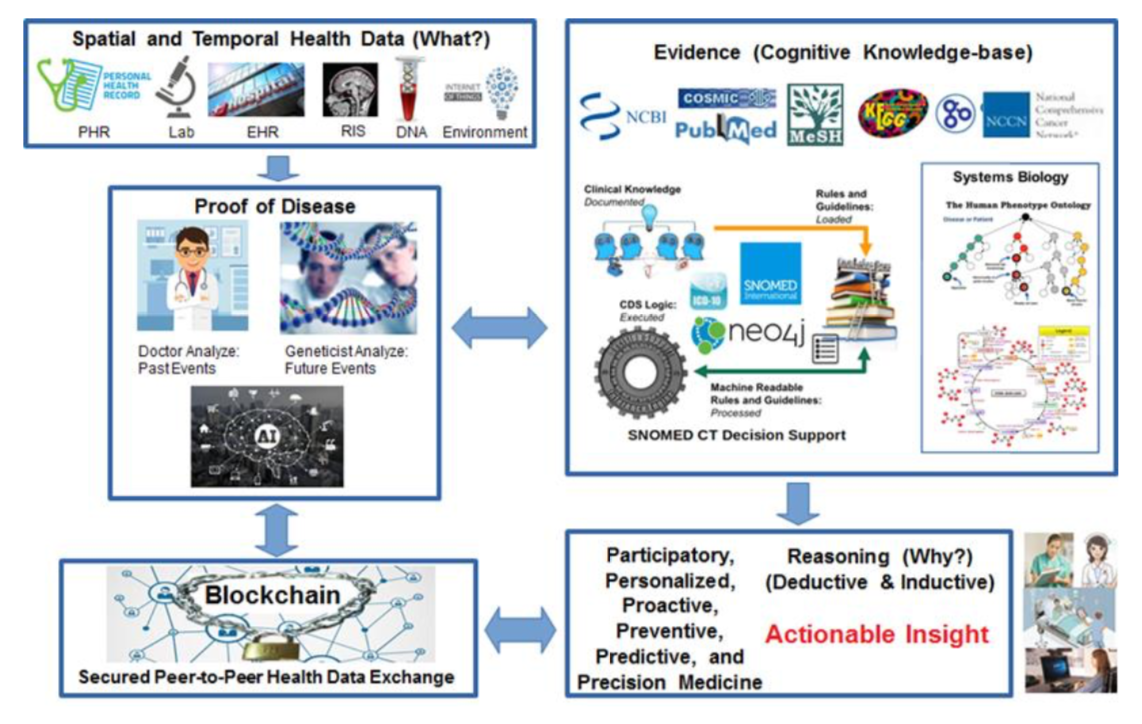
\includegraphics[width=1\textwidth]{images/example_software_architecture.png}
	\caption{Example software architecture cf.\autocite{talukder}}
	\label{example_software_architecture}
\end{figure}
\section{Medical Documentation Apps}

\footnote{cf.\autocite{lupton_mhealth}}
\footnote{cf.\autocite{lupton_apps}}
\footnote{cf.\autocite{akhtar}}
\footnote{cf.\autocite{kawohl}}
\footnote{cf.\autocite{zini}}
\footnote{cf.\autocite{zimmermann}}
https://www.heart.org/en

\begin{figure}[htbp]
	\centering
	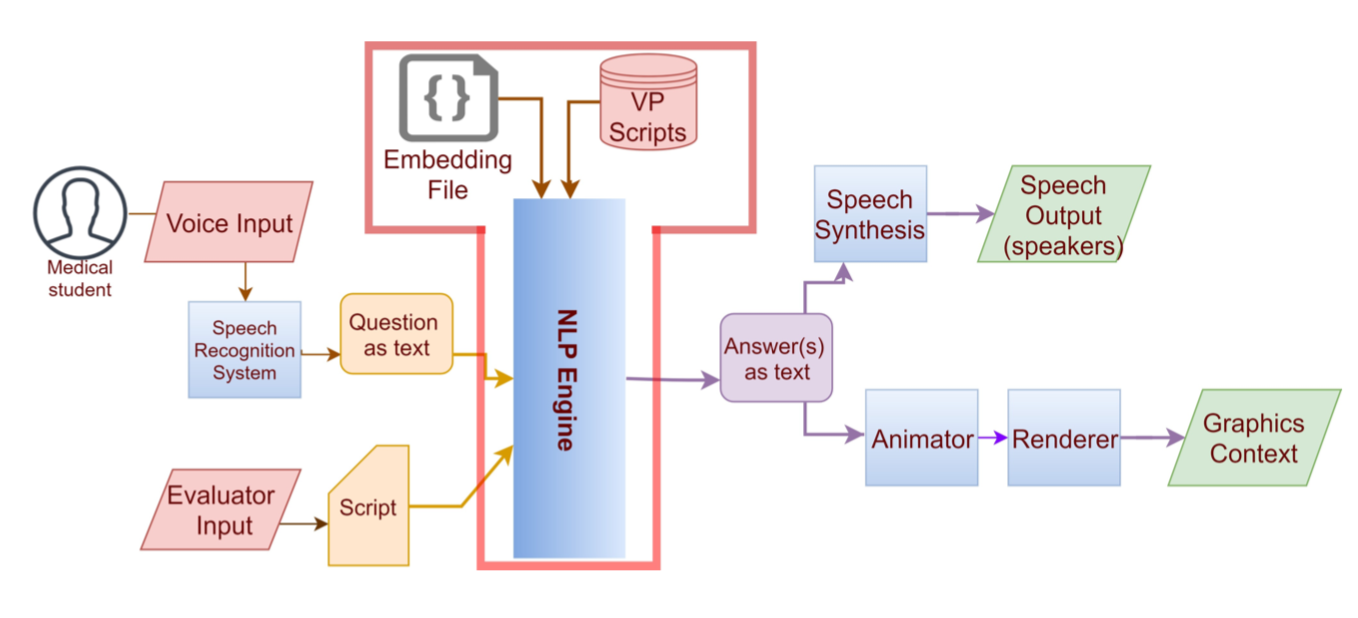
\includegraphics[width=1\textwidth]{images/vp_architecture.png}
	\caption{Virtual patient software architecture cf.\autocite{zini}}
	\label{vp_architecture}
\end{figure}

\begin{figure}[htbp]
	\centering
	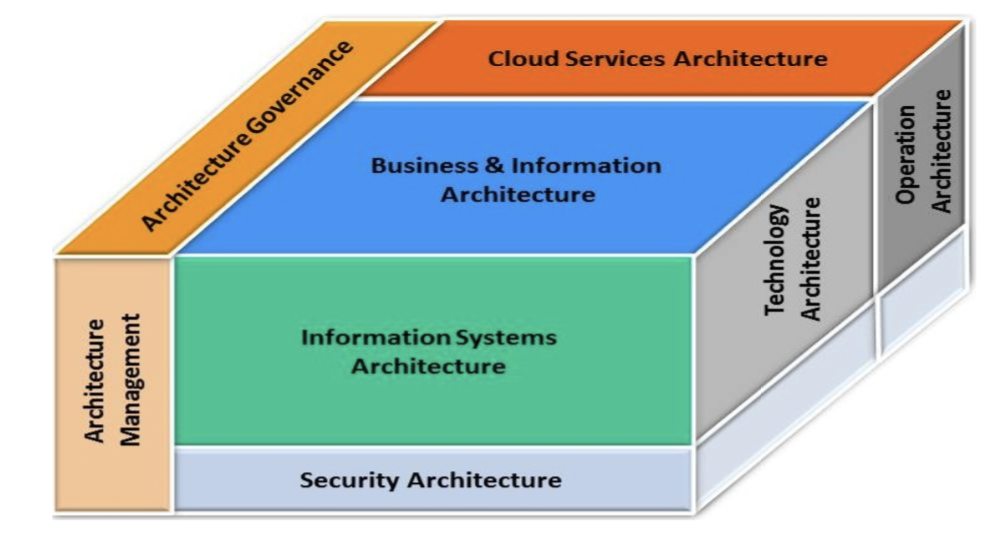
\includegraphics[width=1\textwidth]{images/esarc_cube.png}
	\caption{\ac{esarc} as an example for big data architecture cf.\autocite{zimmermann}}
	\label{vp_architecture}
\end{figure}

\begin{figure}[htbp]
	\centering
	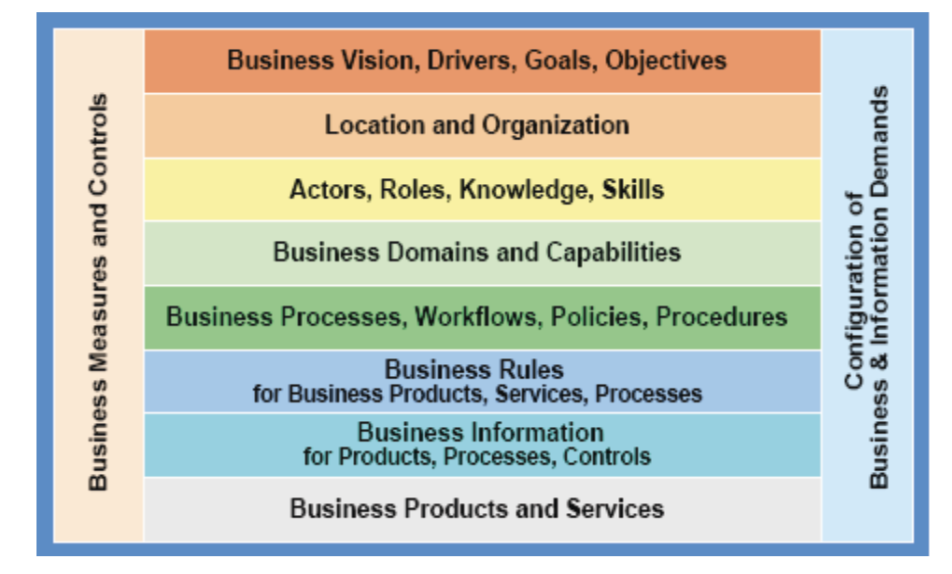
\includegraphics[width=1\textwidth]{images/esarc_business.png}
	\caption{\ac{esarc} business and information reference architecture cf.\autocite{zimmermann}}
	\label{vp_architecture}
\end{figure}

Blood Pressure Apps:
Was können die schon ? 
%https://freeappsforme.com/apps-to-measure-blood-pressure/#cardio-journal
\section{Chatbots} 




\chapter{Analysis and Development}
First of all, the developed chatbot includes information about blood pressure and was built to remind patients of their measurements. Secondly, based on the measured data, analysis can be done in order to react earlier to outliers. Thirdly, a generated report is sent to the doctor so that he can get more insights about the blood pressure values of his patients and improve the treatment.
One of the main challenges during development was the process of providing information about the disease to the patient. Is it possible to include information about different types of blood pressure into the automated conversation with a chatbot? Or does it overwhelm the conversation's use case? Is it useful to let the user ask questions like: 'What are the different types of hypertension? Am i a high-risk patient?' 
Or should these information be provided as a video or a simple web page with long articles to read? Might the patient or user be aborred after a while of talking to a chatbot who only knows answering his questions in the same way?
Of course, a chatbot can be developed more intelligent to never provide the same answer and to answer more precisely to a users' intent. But this requires a lot of training and testing. 
For that reason, in the first version of this chatbot, five simple intents and dialogs have been designed and implemented with the focus of the instructions to measure correctly and regularly. 
In a second or third version, it is possible to focus more on the improvement of providing information about the disease (by not doing this in the style of question and answering).

\section{Experimental set-up}

\subsection{Software architecture}

\subsection{Components}
\begin{figure}[htbp]
	\centering
	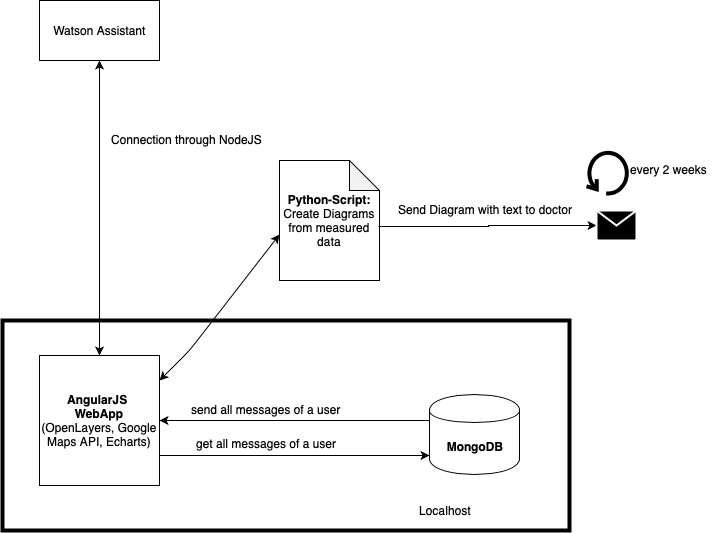
\includegraphics[width=1\textwidth]{images/components.png}
	\caption{Component diagram of developed solution}
	\label{ncbi_query}
\end{figure}

\paragraph{Kaggle Dataset}
%https://www.kaggle.com/mkachuee/BloodPressureDataset
\paragraph{Development of Watson Assistant Dialog}

\subparagraph{Intent model}

The chatbot was built according to the description of "Deutsche Hochdruckliga", a german organization for patients with hypertonia \footnote{cf.\autocite{hochdruckliga}}.
To better understand the users and patients a basic intent model with five intents was developed. 
The five intents include 

%\begin{labeling}{Hypertonie_Messung}
%\item [Hypertonie_Definition] What is hypertonia?
%\item [Hypertonie_Schaeden] What are the consequences of hypertonia?
%\item [Hypertonie_Risiko] How possible is it that i can suffer from hypertonia?
%\item [Hypertonie_Symptome] What are the symptoms of hypertonia?
%\item [Hypertonie_Messung] How can i messure my blood pressure?
%\end{labeling}

These five intents were used to define and develop five typical dialogs.

\paragraph{Setup of MongoDB and basic AngularJS Frontend}

\paragraph{Connect Watson Assistant to Frontend and MongoDB}

\paragraph{Data visualization: Development of a Python Script to show all measured values}

\paragraph{Development of recommendation of nearest doctors to patient}
outlook: maybe in future to connect to the doctors' calendar to directly make an appointment through the chatbot

\paragraph{Development of email service to send reports every two weeks to the doctor}

Another challenge was the way to automatically ask the user for his measured data. A 'usual' chatbot only helps in certain situations including precise user intents, e.g. the question 'When should i measure my blood pressure?'. But they are not constructed to ping a user every five hours or once a day in order to retrieve his measured data, analyze these and send them to a doctor. 
In order to face this problem or use case, a routine including a timer had to be implemented.

\section{Problem solving}
\subsection{Tests}
\subsection{Dataset}
\section{Results}

\chapter{Conclusion and Outlook }
\section{Conclusion}

\section{Outlook}
Is a chatbot an appropriate solution for recording and reminding patients to measure their blood pressure ? 
In practice, most chatbots are created to solve and help multiple intents of their users and not to only 'retrieve' information.
On the one hand, the retrieved information can be used to run several analysis and to find out trends in the data. But on the other hand, the developed solution  supports users to never forget to measure and doctors to better understand trends in the measured data.
During development and research, there came up another issue: To inform patients precisely about their illness. Most patients go to doctors and describe their symptoms, the doctor makes some diagnosis and provides them some medication. But in most cases, doctors do not have enough time to answer all the questions of their patients. For that reason it might be useful to provide a 24/7 service for patients with chronic disease to both record their symptoms and measurements and to answer all their questions.


connection frontend (angularjs webpage) to mongodb through socket.io connection.
Connection between Watson Assistant and Frontend through mongodb and via socket.io connection.


% ncbi query for all genomes
%\begin{figure}[htbp]
%	\centering
	%\includegraphics[width=1\textwidth]{Image/ncbi_all_result.png}
%	\caption{\ac{ncbi} query to find all \ac{all} related gene sequences}
%	\label{ncbi_query}
%\end{figure}


\chapter{Abbreviations}
\begin{acronym}[ARIMA]
\acro{arima}[ARIMA]{Autoregressive Integrated Moving Average Model}
\acro{nlp}[NLP]{Natural Language Processing}
\acro{esarc}[ESARC]{Enterprise Software Architecture Reference Cube}
\acro{m-health}[M-HEALTH]{medical health}
\end{acronym}
\printbibliography

\chapter{Appendix A}\label{appendix a}
\ohead[]{Ehrenwörtliche Erklärung \hfill \thepage}

\null\vfill
\textbf{Ehrenwörtliche Erklärung}

Hiermit versichere ich, dass die vorliegende Arbeit von mir selbstständig und ohne unerlaubte Hilfe angefertigt worden ist, insbesondere dass ich alle Stellen, die wörtlich oder annähernd wörtlich aus Veröffentlichungen entnommen sind, durch Zitate als solche gekennzeichnet habe. Ich versichere auch, dass die von mir eingereichte schriftliche Version mit der digitalen Version übereinstimmt. Weiterhin erkläre ich, dass die Arbeit in gleicher oder ähnlicher Form noch keiner Prüfungsbehörde / Prüfungsstelle vorgelegen hat. Ich erkläre mich damit nicht einverstanden, dass die Arbeit der Öffentlichkeit zugänglich gemacht wird. Ich erkläre mich damit einverstanden, dass die Digitalversion dieser Arbeit zwecks Plagiatsprüfung auf die Server externer Anbieter hochgeladen werden darf. Die Plagiatsprüfung stellt keine Zurverfügungstellung für die Öffentlichkeit dar.

\ \\ \ \\ 


Ort, Datum (Vorname Nachname)

\vfill
\chapter{Appendix B}\label{appendix b}
%\includepdf[pages=-]{lda_all_genomes_v04.pdf}

\end{document}
